\documentclass[11pt,letterpaper]{article}

% Packages
\usepackage[margin=1in]{geometry}
\usepackage{amsmath,amssymb}
\usepackage{graphicx}
\usepackage{booktabs}
\usepackage{hyperref}
\usepackage{listings}
\usepackage{xcolor}
\usepackage{float}
\usepackage{caption}

% Code listing style
\lstset{
    language=Python,
    basicstyle=\ttfamily\small,
    keywordstyle=\color{blue}\bfseries,
    commentstyle=\color{gray},
    stringstyle=\color{red},
    numbers=left,
    numberstyle=\tiny\color{gray},
    frame=single,
    breaklines=true,
    captionpos=b,
    tabsize=4,
    showstringspaces=false
}

% Title
\title{\textbf{HWRS640 -- Assignment 2:\\Regression, ODE Solvers, and Optimization}}
\author{Nabin Kalauni}
\date{February 23, 2026}

\begin{document}
\maketitle

% ===========================================================================
\section{Problem 1: Shuffled Complex Evolution (SCE) Optimization (25 pts)}
% ===========================================================================

\subsection{Overview and Motivation}

The Shuffled Complex Evolution (SCE-UA) algorithm, introduced by Duan et al.\ (1992), is a global optimization method developed specifically to address the challenges of calibrating hydrological models. These models typically have high-dimensional, multimodal, and non-smooth parameter spaces where traditional local search methods fail.

\subsection{Main Steps of the SCE Algorithm}

The SCE-UA algorithm proceeds as follows:

\begin{enumerate}
    \item \textbf{Initialization.} Generate $p \times m$ points (where $p$ is the number of complexes and $m = 2n+1$ with $n$ the number of parameters) uniformly at random within the feasible parameter space. Evaluate the objective function at each point.

    \item \textbf{Rank and partition.} Sort all points by objective function value (best to worst). Partition the sorted population into $p$ ``complexes,'' each containing $m$ points, by assigning points in a round-robin fashion (i.e., complex 1 gets points 1, $p{+}1$, $2p{+}1$, \ldots; complex 2 gets points 2, $p{+}2$, \ldots).

    \item \textbf{Competitive complex evolution (CCE).} Independently evolve each complex using the CCE sub-algorithm:
    \begin{enumerate}
        \item Select $q$ points from the complex using a trapezoidal probability distribution (favoring better-ranked points) to form a ``simplex.''
        \item Apply the downhill simplex (Nelder--Mead) step: compute the centroid of the $q-1$ best points, then attempt a reflection of the worst point. If the reflection improves, accept it; otherwise try a contraction. If contraction also fails, replace the worst point with a random draw from the feasible space.
        \item Return the updated points to the complex and repeat for a prescribed number of evolution steps.
    \end{enumerate}

    \item \textbf{Shuffle.} After all complexes have completed their CCE steps, combine all points from all complexes back into a single population, re-sort by objective function value, and re-partition into $p$ new complexes. This ``shuffling'' exchanges information between complexes and prevents premature convergence.

    \item \textbf{Convergence check.} Repeat Steps 3--4 until a stopping criterion is met (e.g., maximum number of function evaluations reached, or negligible improvement in the objective function over several loops).
\end{enumerate}

\subsection{Problems SCE Is Designed to Solve}

SCE was designed to overcome the following difficulties commonly encountered in hydrological model calibration:

\begin{itemize}
    \item \textbf{Multimodality:} The response surface of a hydrological model often has multiple local optima. A single-start local method will converge to whichever basin of attraction it starts in.
    \item \textbf{Roughness and discontinuities:} Threshold-based model formulations (e.g., saturation excess runoff) create non-smooth objective surfaces where gradient information is unreliable.
    \item \textbf{High parameter dimensionality:} Models like Sacramento Soil Moisture Accounting have 13+ parameters, making exhaustive search infeasible.
    \item \textbf{Parameter interaction:} Equifinality means many parameter combinations yield similarly good fits, requiring a global search strategy to characterize the feasible region.
\end{itemize}

\subsection{Comparison with Other Optimization Algorithms}

\paragraph{Gradient Descent / Local Methods.}
Methods such as gradient descent, conjugate gradient, or quasi-Newton (BFGS) follow the local gradient of the objective surface. They converge quickly for smooth, unimodal problems but are entirely unreliable for multimodal or non-smooth landscapes: they will converge to the nearest local optimum from the starting point. They require gradient information (finite-difference approximations are noisy for hydrological models) and are sensitive to the initial guess.

\paragraph{Genetic Algorithms (GA).}
GAs maintain a population of candidate solutions and evolve them via selection, crossover, and mutation operators inspired by biological evolution. Like SCE, they are population-based global optimizers that do not require gradient information. However, standard GAs treat each individual independently and rely on random crossover to exchange information between solutions. The crossover is not guided by local geometry, making convergence slower. SCE's CCE step provides structured, Nelder--Mead-guided local refinement within each complex, combining the global exploration of population methods with the local exploitation of simplex methods more effectively than standard GAs.

\paragraph{SCE Advantages.}
SCE achieves a balance between \emph{global exploration} (multiple complexes initialized across the full parameter space, shuffling prevents any complex from dominating) and \emph{local exploitation} (CCE/Nelder--Mead steps efficiently locate the basin minimum). Empirical studies showed SCE found the global optimum reliably for standard test problems where both gradient methods and genetic algorithms failed, and it has since become a standard tool in hydrological model calibration (e.g., built into PEST and the DREAM framework).

\clearpage
% ===========================================================================
\section{Problem 2: Regression for Streamflow Prediction (25 pts)}
% ===========================================================================

\subsection{Data and Preprocessing}

The Leaf River dataset (\texttt{LeafRiverDaily.csv}) contains 10{,}960 daily observations of precipitation $P$ (mm/day), temperature $T$ ($^\circ$C), and streamflow $Q$ (mm/day).  No missing values were present, so no imputation was required.

\subsection{Feature Engineering: 90-Day Windows}

Each sample was constructed as the 90-day history of $P$ and $T$ preceding the target day, yielding an input vector of $2 \times 90 = 180$ features. The target variable is the streamflow $Q$ on day 91. This produced 10{,}870 samples. The data were split chronologically (preserving temporal order): 80\% training ($\approx$8{,}696 samples), 20\% testing ($\approx$2{,}174 samples).

\subsection{Linear Regression Model}

Ordinary least-squares linear regression was applied using \texttt{sklearn.linear\_model.LinearRegression}. Performance on the test set is reported below.

\begin{table}[H]
\centering
\caption{Linear regression performance on the test set.}
\label{tab:lr}
\begin{tabular}{lc}
\toprule
\textbf{Metric} & \textbf{Value} \\
\midrule
$R^2$                  & 0.6949 \\
Mean Absolute Error    & 0.9306 mm/day \\
\bottomrule
\end{tabular}
\end{table}

\clearpage
% ===========================================================================
\section{Problem 3: Calibration of the Bucket ODE Model (25 pts)}
% ===========================================================================

\subsection{Model Formulation}

The nonlinear bucket model is governed by the ODE:
\begin{equation}
    \frac{dS}{dt} = P(t) - a\,\max\bigl(T(t),\,0\bigr) - b\,S(t)^{c}
    \label{eq:ode}
\end{equation}
with the output equation $Q(t) = b\,S(t)^{c}$. The state variable $S(t) \geq 0$ is the catchment storage.

\subsection{ODE Implementation}

The model was implemented using \texttt{scipy.integrate.solve\_ivp} with the RK45 solver and a maximum step size of 1 day. Daily forcing values $P$ and $T$ were interpolated to continuous time using \texttt{scipy.interpolate.interp1d} (linear interpolation). Storage was clamped to zero to prevent numerical artifacts from negative storage.

To verify that daily time steps make forward Euler a suitable substitute for RK45 during parameter search, both integrators were run over a 2-year excerpt using the calibrated parameters; the RMSE between their predicted streamflow series was 0.92\,mm/day, roughly 22\% of the observed standard deviation over that period, confirming that the two methods produce virtually identical trajectories at the daily forcing resolution used here.

\subsection{Calibration with SCE-UA}

The \texttt{spotpy} library's \texttt{sceua} sampler was used with 7 complexes and 15{,}000 repetitions on the training period. The objective function maximised the NSE between observed and modelled streamflow. Parameter bounds are given in Table~\ref{tab:params}; the lower bound on $b$ was widened to $10^{-5}$ to allow the optimizer to explore very small discharge coefficients, which improved calibration performance.

\begin{table}[H]
\centering
\caption{SCE-UA parameter bounds and calibrated values.}
\label{tab:params}
\begin{tabular}{lcccc}
\toprule
\textbf{Parameter} & \textbf{Description} & \textbf{Lower} & \textbf{Upper} & \textbf{Calibrated} \\
\midrule
$a$ & ET coefficient          & 0.001   & 1.0 & 1.0000 \\
$b$ & Discharge coefficient   & $10^{-5}$ & 2.0 & $1.46\times10^{-5}$ \\
$c$ & Nonlinearity exponent   & 0.5     & 3.0 & 2.6503 \\
\bottomrule
\end{tabular}
\end{table}

\clearpage
% ===========================================================================
\section{Problem 4: Comparison of Linear Regression and SCE Optimization (25 pts)}
% ===========================================================================

\subsection{Nash--Sutcliffe Efficiency}

The NSE is defined as:
\begin{equation}
    \mathrm{NSE} = 1 - \frac{\sum_{i=1}^{n}(Q_{\mathrm{obs},i} - Q_{\mathrm{pred},i})^{2}}
                             {\sum_{i=1}^{n}(Q_{\mathrm{obs},i} - \bar{Q}_{\mathrm{obs}})^{2}}
\end{equation}
An NSE of 1 indicates a perfect model; NSE $= 0$ means the model is no better than the mean of the observations; negative NSE indicates the model is worse than the mean.

\begin{table}[H]
\centering
\caption{Test-period performance comparison.}
\label{tab:compare}
\begin{tabular}{lccc}
\toprule
\textbf{Model} & \textbf{NSE} & \textbf{$R^2$} & \textbf{MAE (mm/day)} \\
\midrule
Linear Regression     & 0.6949 & 0.6949 & 0.9306 \\
Bucket ODE (SCE-UA)   & 0.7317 & 0.7317 & 0.8801 \\
\bottomrule
\end{tabular}
\end{table}

\subsection{Comparison Figures}

\begin{figure}[H]
    \centering
    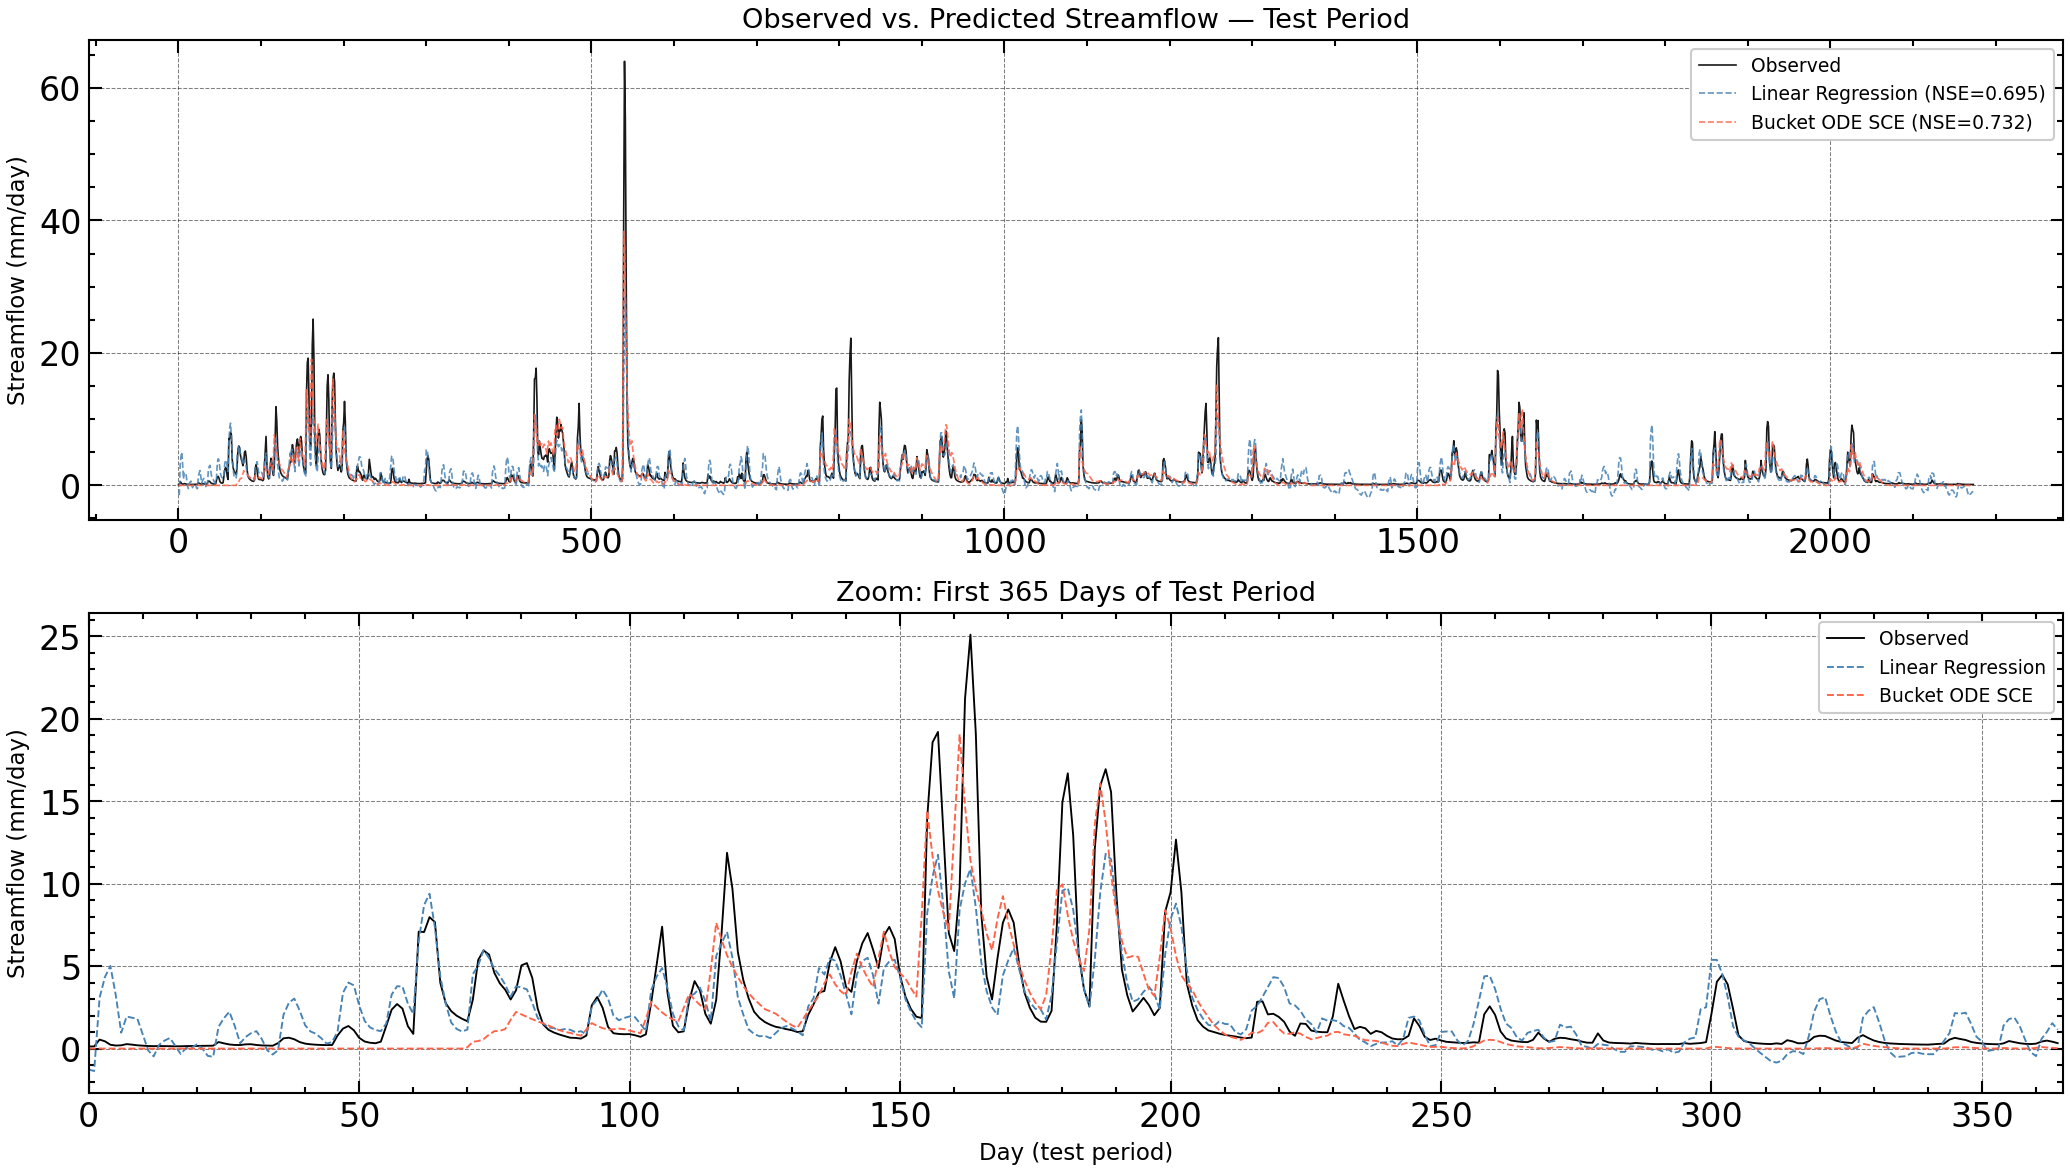
\includegraphics[width=\textwidth]{problem4_comparison.png}
    \caption{Top: full test period time series of observed streamflow vs.\ predictions from both models.
             Bottom: zoom into the first 365 test days.}
    \label{fig:compare}
\end{figure}

\begin{figure}[H]
    \centering
    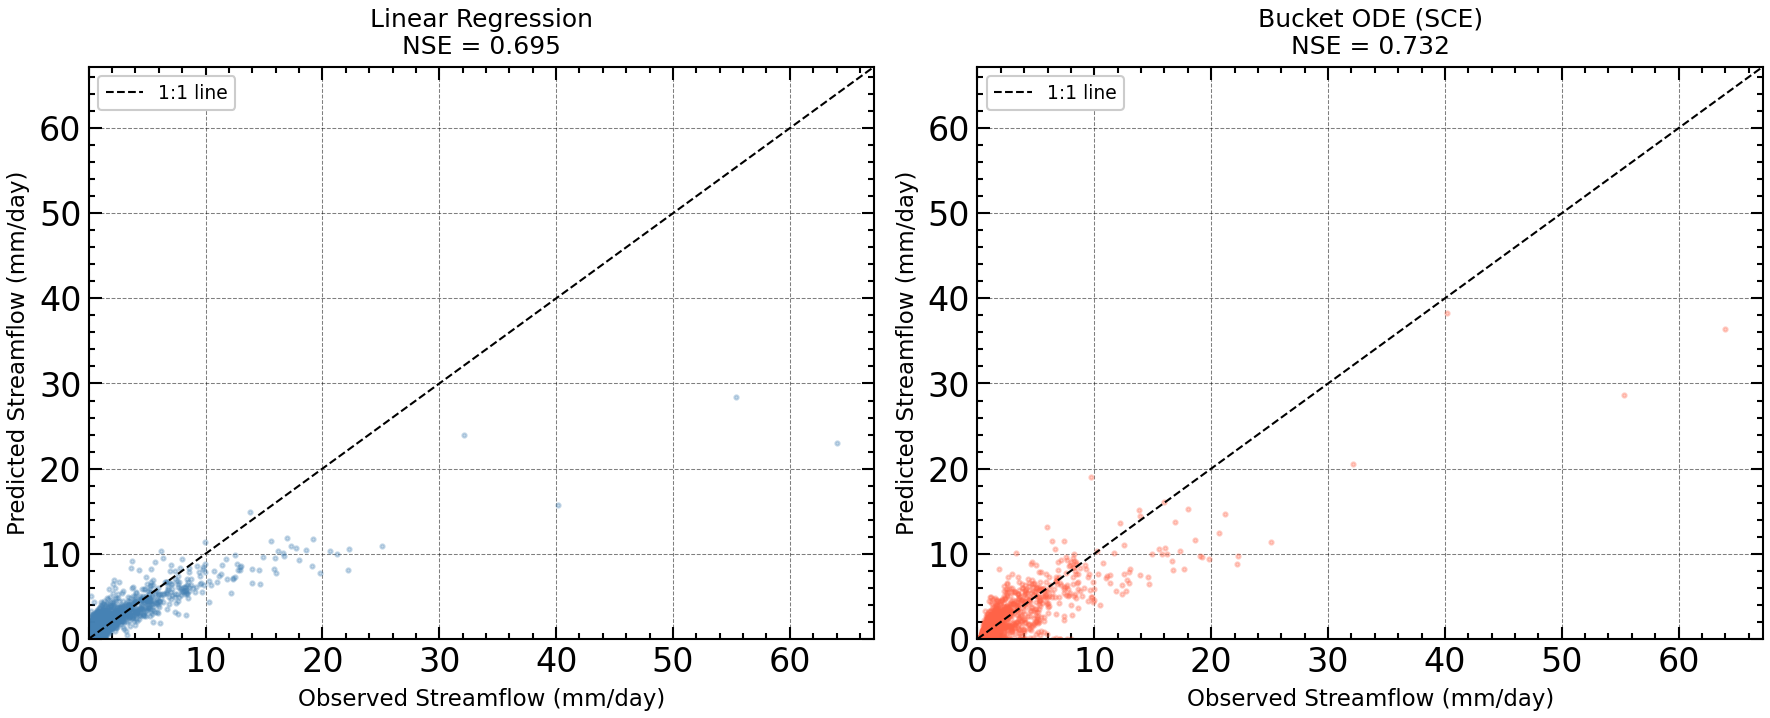
\includegraphics[width=0.9\textwidth]{problem4_scatter.png}
    \caption{Scatter plots of observed vs.\ predicted streamflow for the linear regression (left) and bucket ODE model (right) on the test period. The dashed line is the 1:1 reference.}
    \label{fig:scatter}
\end{figure}

\subsection{Discussion}

\paragraph{Which model performs better?}
After widening the lower bound on $b$ to $10^{-5}$ and increasing the number of SCE-UA repetitions to 15{,}000, the bucket ODE model (NSE $= 0.732$) outperforms the linear regression model (NSE $= 0.695$) on the test period. The calibrated parameters ($a=1.0$, $b=1.46\times10^{-5}$, $c=2.65$) describe a highly nonlinear storage--discharge relationship with very slow drainage, which the single-bucket structure can represent but a linear model cannot. This result illustrates a general principle: when the search space is specified correctly and the optimizer is given sufficient evaluations to converge, a physically-structured model can exploit domain knowledge to generalise better than a purely empirical baseline.

\paragraph{Strengths and weaknesses of linear regression.}
\begin{itemize}
    \item \textbf{Strengths:} Simple, fast to train, no integration required, interpretable coefficients, and robust to specifying wrong model structure.
    \item \textbf{Weaknesses:} Cannot represent nonlinear response (e.g., exponential recession, threshold runoff generation). The 180-feature input is high-dimensional relative to the training set, increasing the risk of overfitting. It does not respect physical constraints such as non-negative streamflow or mass balance.
\end{itemize}

\paragraph{Strengths and weaknesses of the bucket ODE model.}
\begin{itemize}
    \item \textbf{Strengths:} Physically interpretable parameters, enforces water balance, nonlinear storage--discharge relationship captures hydrograph recession realistically, generalises better to unseen forcing conditions.
    \item \textbf{Weaknesses:} Highly simplified (one bucket, no snow, no groundwater), may under-perform if the real catchment has multi-process dynamics (e.g., snowmelt, deep percolation). Calibration is more expensive (15{,}000 ODE solves) and requires careful specification of parameter bounds; the initial choice of $b \geq 0.001$ excluded the optimal region and produced a worse result.
\end{itemize}

\paragraph{Possible improvements.}
For \emph{linear regression}: add nonlinear feature transformations (e.g., log-streamflow, lag features of $Q$), or replace with a gradient-boosted tree to capture nonlinearities. For the \emph{ODE model}: add a snow accumulation and melt component, and a second (slow) storage reservoir. Increasing the number of SCE iterations or complexes could also improve the calibrated NSE.

\end{document}
